\chapter{Fundamentos Teóricos}
\label{ch:fund-teor}
%
Do modo a se colmatar as necessidades teóricas para o desenvolvimento do robô foram estudadas as seguintes ferramentas: 

\underline{\textit{Autodesk Fusion 360}}, uma excelente ferramenta \textit{CAD} para a modelação precisa de objetos 2D e 3D. Na qual, existem vários ambientes de trabalho, cada um fornecendo ao utilizador características e opções distintas. O ambiente de trabalho usado por defeito nesta ferramenta é o \textit{Design}, sendo possível alterar a qualquer altura.  

Neste ambiente de trabalho, a modelação 3D de um objeto é inicialmente feita usando esboços. Primeiro, é feita a escolha de um plano para o esboço e, em seguida desenhado o esboço 2D recorrendo a funcionalidades como linhas, curvas e outros elementos 2D simples. Por fim, é possível adicionar espessura ao esboço de modo a criar um objeto 3D. 

Este ambiente de trabalho permite também a criação de vários objetos em ficheiros separados, que podem ser juntos ou não num novo ficheiro. 

\textit{\underline{CoppeliaSim}}, ferramenta muito usada na educação relacionada com robótica, principalmente a nível de criação de modelos físicos e ambientes de simulação. 

Dada a complexidade das formas criadas em \textit{CAD}, um ficheiro \textit{CAD} não é normalmente usado também como modelo físico uma vez que tornaria este demasiado complexo. Sendo desta forma, vantajoso a procura da criação de um modelo físico mais básico usando o \textit{CoppeliaSim}. 

A criação de um modelo fisíco através do \textit{CoppeliaSim} pode ser realizada recorrendo a diversas formas primitivas como, \textit{plane, disc, cuboid, sphere} e \textit{cylinder}, e/ou a modelos pré-criados. Devendo peças que terão movimento relativamente a outras serem colocadas separadamente e hierarquicamente na \textit{scene hierarchy}. 

De modo a complementar o modelo físico criado em \textit{CoppeliaSim}, é possível utilizar o modelo gráfico criado em \textit{CAD} tornado assim o modelo mais apelativo visualmente e simplista fisicamente. Esta junção implica que ficheiros \textit{CAD} sejam gravados com formatos interpretados pelo \textit{CoppeliaSim}, como \textit{obj, dxf, ply} e \textit{stl} de modo a serem posteriormente importados e realizada a \textit{mesh}.  

\underline{Navegação autónoma}, exige a criação de algoritmos de modo a tornar possíveis vários fatores essenciais no seu processo, tais como: 
\begin{itemize}
    \item Navegação na direção de uma posição alvo (\textit{target acquisition});
    \item Evitar colisões com obstáculos (\textit{obstacle avoidance}); 
    \item Integração do comportamento de navegação na direção de uma posição alvo e evitar colisões com obstáculos (dinâmica não-linear); 
    \item Integração do comportamento de navegação na direção de uma posição alvo e evitar colisões com obstáculos (dinâmica linear). 
\end{itemize}

Em respeito ao \underline{\textit{Target acquisition}}, um robô móvel autónomo para ser útil tem que ser capaz de navegar para uma posição alvo. A informação sobre o alvo pode ser definida pelas coordenadas do alvo (x\textsubscript{alvo}, y\textsubscript{alvo}) ou o sistema de visão pode indicar em que direção está a detetar o alvo (Figura \ref{fig:obs-e-target}).

Dinâmica de navegação:

\begin{figure*}[!h]
\centering
    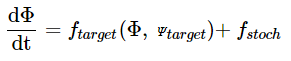
\includegraphics[width=0.3\textwidth]{./img/eq-1.1}
    \caption*{Equação (1.1)}
\label{eq:1.1}
\end{figure*}

Onde,
%
\begin{figure*}[!h] 
\centering
    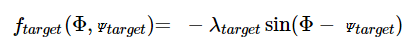
\includegraphics[width=0.5\textwidth]{./img/eq-1.2}
    \caption*{Equação (1.2)}
\label{eq:1.2}
\end{figure*}

Dinâmica da velocidade linear: 

\begin{figure*}[!h]
\centering
    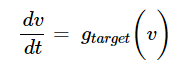
\includegraphics[width=0.2\textwidth]{./img/eq-1.3}
    \caption*{Equação (1.3)}
\label{eq:1.3}
\end{figure*}
%
\begin{figure}[!h]
\centering
    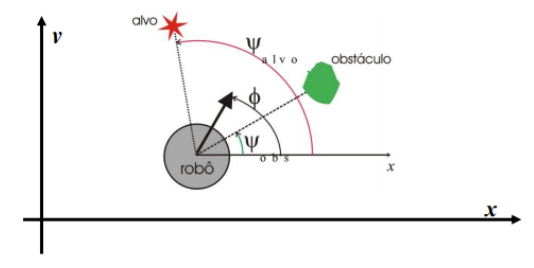
\includegraphics[width=0.7\textwidth]{./img/obs-e-target}
    \caption{Ângulo segundo o qual o robot "vê", $\psi$\textsubscript{target}, o alvo em relação ao sistema dos eixos coordenados do mundo pode ser dado pelo sistema de visão do robot ou ser calculado se as coordenadas do alvo, (X\textsubscript{target},Y\textsubscript{target}),  forem conhecidas e se tiver.}
\label{fig:obs-e-target}
\end{figure}

Através do estudo analítico dos sistemas dinâmicos é possível a atribuição de valores adequados aos seus parâmetros por forma a que os atractores surjam com os devidos valores, e que simultaneamente as variáveis de estado consigam seguir de perto um atractor à medida que este se desloca. Contribuindo assim para a estabilidade assimptótica do sistema que gera o comportamento do robô e o torna mais robusto face a perturbações externas. 

O método de \textit{Lyapunov} é um método que consiste em encontrar uma função 
U(x) continuamente diferenciável, chamada função de \textit{Lyaponov}, representando a ‘energia’ do sistema. No qual, através desta função é possível investigar a estabilidade dos pontos fixos de um sistema dinâmico.  

Considerando o \underline{conceito de ‘energia’} e olhando para o sistema dinâmico como se fosse um sistema físico dissipativo, isto é, sendo uma função que a cada estado do sistema x associa uma quantidade de energia potencial U(x). Se o sistema for tal que perde energia ao longo do tempo, e a energia perdida nunca é restabelecida (figura \ref{fig:ex-energia}) verifica-se que

%
\begin{figure*}[!h]
\centering
    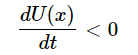
\includegraphics[width=0.15\textwidth]{./img/eq-1.4}
    \caption*{Equação (1.4)}
\label{eq:1.4}
\end{figure*}

e que eventualmente o estado do sistema vai acabar por parar e ficar num estado de repouso final x*(atrator). Neste, se o estado do sistema deixa de variar, então também a sua energia deixa de variar, pelo que se verifica
%
\begin{figure*}[!h] 
\centering
    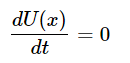
\includegraphics[width=0.15\textwidth]{./img/eq-1.5}
    \caption*{Equação (1.5)}
\label{eq:1.5}
\end{figure*}

\begin{figure}[!h]
\centering
    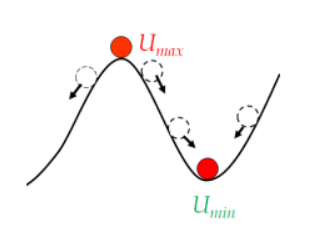
\includegraphics[width=0.4\textwidth]{./img/ex-energia.png}
    \caption{ O sistema perde energia ao longo do tempo. O estado do sistema vai acabar por parar e ficar num estado de repouso final x* (atrator).}
\label{fig:ex-energia}
\end{figure}

Tendo em consideração agora o \texttt{conceito de sistema dinâmico gradiente}, i.e. um sistema cujo campo vetorial resulta do gradiente de uma função:
%
\begin{figure*}[!h] 
\centering
    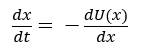
\includegraphics[width=0.2\textwidth]{./img/eq-1.6-1}
\label{eq:1.6-1}
\end{figure*}


ou seja
%
\begin{figure*}[!h]
\centering
    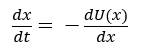
\includegraphics[width=0.2\textwidth]{./img/eq-1.6-1}
    \caption*{Equação (1.6)}
\label{eq:1.6}
\end{figure*}

Cruzando ambos os conceitos obtém-se que
%
\begin{figure*}[!h]
\centering
    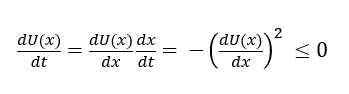
\includegraphics[width=0.45\textwidth]{./img/eq-1.7}
    \caption*{Equação (1.7)}
\label{eq:1.7}
\end{figure*}

Ou seja, ao longo do tempo a energia U(t) diminui ao longo de toda a trajetória x(t), por conseguinte a evolução do sistema é sempre no sentido de evoluir para um estado de menor energia.

Adicionalmente, repare-se que
 %
\begin{figure*}[!h]
\centering
    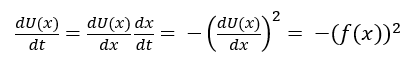
\includegraphics[width=0.5\textwidth]{./img/eq-1.8}
    \caption*{Equação (1.8)}
\label{eq:1.8}
\end{figure*}

Assim, se o sistema for colocado nos pontos de equilíbrio ou pontos fixos x* então a energia do sistema não varia,
%
\begin{figure*}[!h]
\centering
    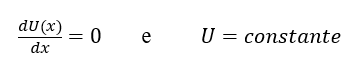
\includegraphics[width=0.45\textwidth]{./img/eq-1.9}
    \caption*{Equação (1.9)}
\label{eq:1.9}
\end{figure*}

Isto porque, nos pontos fixos x* temos
%
\begin{figure*}[!h]
\centering
    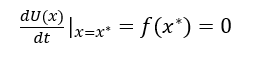
\includegraphics[width=0.35\textwidth]{./img/eq-1.10}
    \caption*{Equação (1.10)}
\label{eq:1.10}
\end{figure*}

\section{Estudo analítico do sistema dinâmico não linear, definido por (1.1) e (1.2):}

Sabidos os pontos físicos do sistema dinâmico (1.1) admitindo que f\textsubscript{target} é definido por (1.3),
%
\begin{figure*}[!h]
\centering
    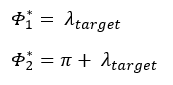
\includegraphics[width=0.25\textwidth]{./img/1.11}
\label{eq:1.11}
\end{figure*}

A sua estabilidade é classificada como:
%
\begin{figure*}[!h]
\centering
    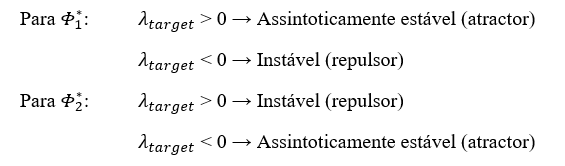
\includegraphics[width=0.65\textwidth]{./img/estabilidade}
\label{eq:estabilidade}
\end{figure*}

Logo, para o robô ter o comportamento desejado, uma vez que o alvo funciona como um ponto fixo atractor e o robô desloca-se para o alvo,

$\lambda$\textsubscript{target} > 0

Sabendo também que a constante de tempo $\tau$ = 1/$\lambda$\textsubscript{target},

$\uparrow \lambda$\textsubscript{target} $\rightarrow  \downarrow \tau$

Mais rapidamente converge o valor de $\phi$ para o atrator.

\section{Estudo analítico do sistema dinâmico linear, definido por (1.11)}

%
\begin{figure*}[!h] 
\centering
    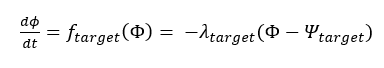
\includegraphics[width=0.5\textwidth]{./img/eq-1.11}
    \caption*{Equação (1.11)}
\label{eq:1.11}
\end{figure*}

Sabidos os pontos físicos do sistema dinâmico,

$\phi* = \psi$\textsubscript{target} 

A sua estabilidade é classificada como: 
%
%
\begin{figure*}[!h]
\centering
    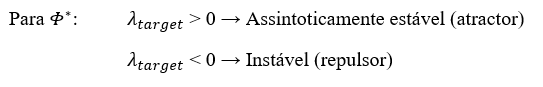
\includegraphics[width=0.6\textwidth]{./img/estabilidade-2}
\label{eq:estabilidade-2}
\end{figure*}
%
Em respeito ao \textit{obstacle avoidance}, um robot móvel autónomo para ser capaz evitar obstáculos recorre a sensores que sejam capazes de detetar as obstruções que aparecem nas suas direções. Detetados os obstáculos, os sensores permitem também estimar a distância a que o robot se encontra destes (figura \ref{fig:sensores}). O controlo do movimento do robot na direção do alvo é realizado através de sistemas dinâmicos para a direção de navegação e velocidade linear.

%
\begin{figure}[!h]
\centering
    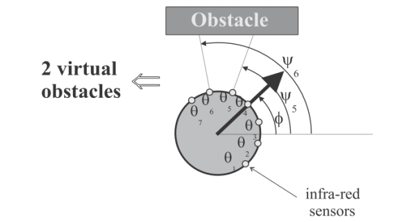
\includegraphics[width=0.5\textwidth]{./img/sensores}
    \caption{Representação do comportamento dos sensores do Robot.}
\label{fig:sensores}
\end{figure}
%
Dinâmica de navegação:
%
\begin{figure*}[!h]
\centering
    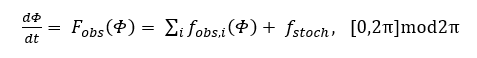
\includegraphics[width=0.6\textwidth]{./img/eq-2.1}
    \caption*{Equação (2.1)}
\label{eq:eq-2.1}
\end{figure*}

Onde,

\begin{figure*}[!h]
\centering
    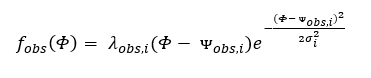
\includegraphics[width=0.5\textwidth]{./img/eq-2.2}
    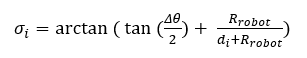
\includegraphics[width=0.4\textwidth]{./img/eq-2.3}
    \caption*{Equação (2.2) e (2.3)}
\label{eq:eq-2.2}
\end{figure*}
%
%\begin{figure*}[!h] 
%\centering
%    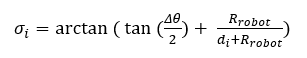
\includegraphics[width=0.4\textwidth]{./img/eq-2.3}
%    \caption*{Equação (2.3)}
%\label{eq:eq-2.3}
%\end{figure*}
%

\begin{figure*}[!h]
\centering
    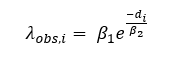
\includegraphics[width=0.25\textwidth]{./img/eq-2.4}
    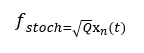
\includegraphics[width=0.25\textwidth]{./img/eq-2.5}
    \caption*{Equações (2.4) e (2.5)}
\label{eq:eq-2.4}
\end{figure*}
%
%\begin{subfigure}
%\centering
%    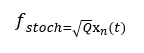
\includegraphics[width=0.25\textwidth]{./img/eq-2.5}
%\label{eq:eq-2.5}
%\end{subfigure}
%\end{figure*}
Uma vez mais, através do estudo analítico dos sistemas dinâmicos é possível a atribuição de valores adequados aos seus parâmetros por forma a que, neste caso, os repulsores surjam com os devidos valores.

\section{Estudo analítico do sistema dinâmico não linear para o comportamento de evitar obstáculos:}

Sabidos os pontos físicos do sistema dinâmico (2.1) quando apenas 1 obstrução, f\textsubscript{obs,i}, é detetada 

$\phi$ = $\psi$\textsubscript{obs,i} 

A sua estabilidade é classificada como:
%
\begin{figure*}[!h]
\centering
    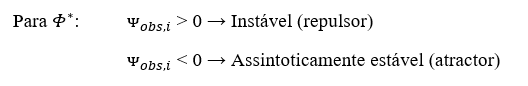
\includegraphics[width=0.7\textwidth]{./img/estabilidade-3}
\label{eq:estabilidade-3}
\end{figure*}

Sabendo também que a constante de tempo $\tau$ = 1/$\psi$\textsubscript{obs,i} ,

$\downarrow$ $\psi$\textsubscript{obs,i} $\rightarrow$ $\uparrow$  $\lambda$\textsubscript{target} $\rightarrow  \uparrow \tau$

Mais rapidamente converge o sistema para o ponto fixo.


Logo, uma vez que o objetivo é o robô desviar-se dos obstáculos, para o robô ter o comportamento desejado o ponto de equilíbrio tem de ser um repulsor. 
%
\begin{figure*}[!h]
\centering
    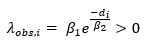
\includegraphics[width=0.25\textwidth]{./img/lambda-obs}
\label{eq:lambda-obs}
\end{figure*}

Onde $\lambda$(obs,i) depende da distância (di) e do parâmetro $\beta$\textsubscript{1},
%
\begin{figure*}[!h]
\centering
    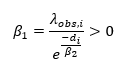
\includegraphics[width=0.25\textwidth]{./img/beta-1}
\label{eq:beta-1}
\end{figure*}

Para se calcular o valor máximo de $\beta$\textsubscript{1} temos de calcular $\lambda$\textsubscript{obs\_max}, 

\begin{figure*}[!h]
\centering
    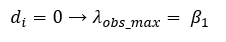
\includegraphics[width=0.4\textwidth]{./img/di}
\label{eq:di}
\end{figure*}

Concluindo que para que o robot tenha o comportamento desejado, o parâmetro $\beta$1 tem de assumir o valor de,

\begin{figure*}[!h]
\centering
    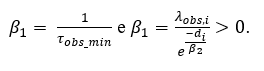
\includegraphics[width=0.4\textwidth]{./img/beta-1-2}
\label{eq:beta-1-2}
\end{figure*}

Em respeito à integração do comportamento de navegação na direção de uma posição alvo e evitar colisões com obstáculos (dinâmica não-linear e dinâmica linear), consiste na integração dos dois fatores anteriores, o target \textit{acquistion} e o \textit{obstacle avoidance}.

\textit{Matlab}, é uma excelente plataforma de programação para o desenvolvimento de algoritmos e criação de modelos.

Através da alteração de \textit{scripts Matlab} é possível a ligação a ambientes de simulação e modelos criados em \textit{CoppeliaSim}. Sendo estas alterações realizadas no construtor de classes, onde são inicializados os \textit{handles}.
